\documentclass[11pt,twoside,a4paper,openright]{report}
%%%%%%%%%%%%%%%%%%%%%%%%%%%%%%%%%%%%%%%%%%%%%%%%
% Language, Encoding and Fonts
% http://en.wikibooks.org/wiki/LaTeX/Internationalization
%%%%%%%%%%%%%%%%%%%%%%%%%%%%%%%%%%%%%%%%%%%%%%%%
% Select encoding of your inputs. Depends on
% your operating system and its default input
% encoding. Typically, you should use
%   Linux  : utf8 (most modern Linux distributions)
%            latin1 
%   Windows: ansinew
%            latin1 (works in most cases)
%   Mac    : applemac
% Notice that you can manually change the input
% encoding of your files by selecting "save as"
% an select the desired input encoding. 
\usepackage[utf8]{inputenc}
% Make latex understand and use the typographic
% rules of the language used in the document.
\usepackage[danish,english]{babel}
% Use the palatino font
\usepackage[sc]{mathpazo}
\linespread{1.05}         % Palatino needs more leading (space between lines)
% Choose the font encoding
\usepackage[T1]{fontenc}

%%%%%%%%%%%%%%%%%%%%%%%%%%%%%%%%%%%%%%%%%%%%%%%%
% Graphics and Tables
% http://en.wikibooks.org/wiki/LaTeX/Importing_Graphics
% http://en.wikibooks.org/wiki/LaTeX/Tables
% http://en.wikibooks.org/wiki/LaTeX/Colors
%%%%%%%%%%%%%%%%%%%%%%%%%%%%%%%%%%%%%%%%%%%%%%%%
% load a colour package
\usepackage{xcolor}
\definecolor{aaublue}{RGB}{33,26,82}% dark blue
% The standard graphics inclusion package
\usepackage{graphicx}
% Set up how figure and table captions are displayed
\usepackage{caption}
\captionsetup{%
  font=footnotesize,% set font size to footnotesize
  labelfont=bf % bold label (e.g., Figure 3.2) font
}
% Make the standard latex tables look so much better
\usepackage{array,booktabs}
% Enable the use of frames around, e.g., theorems
% The framed package is used in the example environment
\usepackage{framed}

% Adds support for full page background picture
\usepackage[contents={},color=gray]{background}
%\usepackage[contents=draft,color=gray]{background}

%%%%%%%%%%%%%%%%%%%%%%%%%%%%%%%%%%%%%%%%%%%%%%%%
% Mathematics
% http://en.wikibooks.org/wiki/LaTeX/Mathematics
%%%%%%%%%%%%%%%%%%%%%%%%%%%%%%%%%%%%%%%%%%%%%%%%
% Defines new environments such as equation,
% align and split 
\usepackage{amsmath}
% Adds new math symbols
\usepackage{amssymb}
% Use theorems in your document
% The ntheorem package is also used for the example environment
% When using thmmarks, amsmath must be an option as well. Otherwise \eqref doesn't work anymore.
\usepackage[framed,amsmath,thmmarks]{ntheorem}

%%%%%%%%%%%%%%%%%%%%%%%%%%%%%%%%%%%%%%%%%%%%%%%%
% Page Layout
% http://en.wikibooks.org/wiki/LaTeX/Page_Layout
%%%%%%%%%%%%%%%%%%%%%%%%%%%%%%%%%%%%%%%%%%%%%%%%
% Change margins, papersize, etc of the document
\usepackage[
  inner=28mm,% left margin on an odd page
  outer=41mm,% right margin on an odd page
  ]{geometry}
% Modify how \chapter, \section, etc. look
% The titlesec package is very configureable
\usepackage{titlesec}
\titleformat{\chapter}[display]{\normalfont\huge\bfseries}{\chaptertitlename\ \thechapter}{20pt}{\Huge}
\titleformat*{\section}{\normalfont\Large\bfseries}
\titleformat*{\subsection}{\normalfont\large\bfseries}
\titleformat*{\subsubsection}{\normalfont\normalsize\bfseries}
%\titleformat*{\paragraph}{\normalfont\normalsize\bfseries}
%\titleformat*{\subparagraph}{\normalfont\normalsize\bfseries}

% Clear empty pages between chapters
\let\origdoublepage\cleardoublepage
\newcommand{\clearemptydoublepage}{%
  \clearpage
  {\pagestyle{empty}\origdoublepage}%
}
\let\cleardoublepage\clearemptydoublepage

% Change the headers and footers
\usepackage{fancyhdr}
\pagestyle{fancy}
\fancyhf{} %delete everything
\renewcommand{\headrulewidth}{0pt} %remove the horizontal line in the header
\fancyhead[RE]{\small\nouppercase\leftmark} %even page - chapter title
\fancyhead[LO]{\small\nouppercase\rightmark} %uneven page - section title
\fancyhead[LE,RO]{\thepage} %page number on all pages
% Do not stretch the content of a page. Instead,
% insert white space at the bottom of the page
\raggedbottom
% Enable arithmetics with length. Useful when
% typesetting the layout.
\usepackage{calc}

%%%%%%%%%%%%%%%%%%%%%%%%%%%%%%%%%%%%%%%%%%%%%%%%
% Bibliography
% http://en.wikibooks.org/wiki/LaTeX/Bibliography_Management
%%%%%%%%%%%%%%%%%%%%%%%%%%%%%%%%%%%%%%%%%%%%%%%%
\usepackage[backend=bibtex,
  bibencoding=utf8,
  style=numeric-comp
  ]{biblatex}
\addbibresource{bib/mybib}

%%%%%%%%%%%%%%%%%%%%%%%%%%%%%%%%%%%%%%%%%%%%%%%%
% Misc
%%%%%%%%%%%%%%%%%%%%%%%%%%%%%%%%%%%%%%%%%%%%%%%%
% Add bibliography and index to the table of
% contents
\usepackage[nottoc]{tocbibind}
% Add the command \pageref{LastPage} which refers to the
% page number of the last page
\usepackage{lastpage}
% Add todo notes in the margin of the document
\usepackage[
%  disable, %turn off todonotes
  colorinlistoftodos, %enable a coloured square in the list of todos
  textwidth=\marginparwidth, %set the width of the todonotes
  textsize=scriptsize, %size of the text in the todonotes
  ]{todonotes}

%%%%%%%%%%%%%%%%%%%%%%%%%%%%%%%%%%%%%%%%%%%%%%%%
% Hyperlinks
% http://en.wikibooks.org/wiki/LaTeX/Hyperlinks
%%%%%%%%%%%%%%%%%%%%%%%%%%%%%%%%%%%%%%%%%%%%%%%%
% Enable hyperlinks and insert info into the pdf
% file. Hypperref should be loaded as one of the 
% last packages
\usepackage{hyperref}
\hypersetup{%
	pdfpagelabels=true,%
	plainpages=false,%
	pdfauthor={Author(s)},%
	pdftitle={Title},%
	pdfsubject={Subject},%
	bookmarksnumbered=true,%
	colorlinks=false,%
	citecolor=black,%
	filecolor=black,%
	linkcolor=black,% you should probably change this to black before printing
	urlcolor=black,%
	pdfstartview=FitH%
}
% package inclusion and set up of the document

\begin{document}
%frontmatter
\pagestyle{empty} %disable headers and footers
\pagenumbering{roman} %use roman page numbering in the frontmatter

%%%% frontpage %%%%
\pdfbookmark[0]{Front page}{label:frontpage}%
\begin{titlepage}
\vspace*{\fill}

    \begin{center}
    \Huge{\textbf{
      WORKSHEETS% insert your title here
    }}
    \end{center}
    \begin{center}
      \Large{
        % insert your subtitle here
      }
    \end{center}
    \vspace{0.2cm}
   \begin{center}
    {\Large
      Trine Nyholm Kragh \& Laura Nyrup Mogensen% insert names separated by comma
    }\\
    \vspace{0.2cm}
    {\large
      Mathematical Engineering, MATTEK% insert name of study, group number, year-month
    }
   \end{center}
   \vspace{0.2cm}
%% Comment this section in if you are doing Bachelor or Master Project   
   \begin{center}
    {\Large
      Master's Thesis
      %Bachelor Project
    }
   \end{center}
   
  \vfill
  \begin{center}
    
\includegraphics[width=0.2\paperwidth]{AAUgraphics/aau_logo_circle_en}% comment this line in for English version
    %
\includegraphics[width=0.2\paperwidth]{AAUgraphics/aau_logo_circle_da} %comment this line in for Danish version
  \end{center}
\end{titlepage}


%%%%%%%%%%%%%%%%%%%



%\pdfbookmark[0]{Contents}{label:contents}
%\pagestyle{fancy} %enable headers and footers again

%\tableofcontents

%\listoftodos

%mainmatter
\pagenumbering{arabic} %use arabic page numbering in the mainmatter
%\chapter{Introduction}\label{ch:introduction}
Here is the introduction. The next chapter is chapter~\ref{ch:ch2label}.


a new paragraph


\section{Examples}
You can also have examples in your document such as in example~\ref{ex:simple_example}.
\begin{example}{An Example of an Example}
  \label{ex:simple_example}
  Here is an example with some math
  \begin{equation}
    0 = \exp(i\pi)+1\ .
  \end{equation}
  You can adjust the colour and the line width in the {\tt macros.tex} file.
\end{example}

\section{How Does Sections, Subsections, and Subsections Look?}
Well, like this
\subsection{This is a Subsection}
and this
\subsubsection{This is a Subsubsection}
and this.

\paragraph{A Paragraph}
You can also use paragraph titles which look like this.

\subparagraph{A Subparagraph} Moreover, you can also use subparagraph titles which look like this\todo{Is it possible to add a subsubparagraph?}. They have a small indentation as opposed to the paragraph titles.

\todo[inline,color=green]{I think that a summary of this exciting chapter should be added.}

\chapter{Motivation}\label{ch:motivation}
 This chapter accounts for the motivation behind source extraction from an Electroencephalography (EEG). The concept of EEG is introduced along with current applications. The potential and importance of source extraction are considered and related to the hearing aid industry. The commonly applied mathematical model for EEG measurements is presented. Currently applied methods for source extraction are considered leading to a presentation of the current state of the art methods which succeeds to overcome the limitations of previous methods. Lastly the objective of this thesis is specified.          

%%This chapter examines existing literature concerning source recovery from Electroencephalography (EEG) measurements. 
%%At first a motivation for the source recovery problem is given, considering the application within the hearing aid industry. 
%%Further, the state of the art methods are presented followed by a description of the contribution proposed in this thesis.

\section{Introduction to EEG Measurements}\label{sec:EEG}
EEG is an imaging technique used within the medical field. EEG is measuring electric signals on the scalp, caused by brain activity. 
The human central nerve system consist of various nerve cells connecting the neurons within the brain. Nerve cells respond to certain stimuli, for instance a physical stimuli, and transmit informations between neurons.
Generally speaking these activities induce local currents that are transferred throughout the nerve system. 
Several nearby simultaneous activations result in local potential fields, referred to as one signal \textit{source}\cite{EEGsignalprocessing}. 
EEG measurements are provided by a number of metal electrodes, referred to as sensors, carefully placed on the human scalp. 
Each sensor reads the present electrical signals over time.
For the source signal to reach a sensor it has to penetrate the skull, skin and several other thin layers of biological tissue. 
This causes an unknown distortion and reduction of a signal.
It is most likely that the measurement of one sensor is a sum of multiple signals from different sources.
Nor is the range of a single sensor separated from the other sensors. 
Thus the same signal can easily be measured by two or more sensors.
The process of distorsion and mixing of signals is called volume conduction \cite[p. 68]{EEGsignalprocessing} \cite{Van2019}. 
From this it is clarified that EEG measurements  
is a mixture of fluctuating electrical signals originating from brain activities. Due to the mixing and the nature of the signals the true number of sources is generally considered unknown\cite{EEGsignalprocessing}.  
Furthermore, EEG is a subject for interfering noise. Noise signals can occur in the measurements resulting from physical movement of e.g. eyes and jawbone \cite{fundamentalEEG}. The concept of volume conduction is sought illustrated on figure \ref{fig:volumeconduction}.

The source signals are classified within four groups according to the dominant frequency. 
The delta wave ($0.5-4$ Hz) is observed from infants and sleeping adults, the theta wave ($4-8$ Hz) is observed from children and sleeping adults, the alpha wave ($8-13$ Hz) is the most extensively studied brain rhythm, which is induced by an adult laying down with closed eyes. 
Lastly, the beta wave ($13-30$ Hz) is considered the normal brain wave for adults, associated with active thinking, active attention or solving concrete problems \cite[p. 11]{EEGsignalprocessing}. 
An example of EEG measurements within the four categories is illustrated by figure \ref{fig:EEG_example}.   

Generally, the distribution of EEG measurements of multiple sensors are considered multivariant Gaussian\todo{does this comply to the non-gaussian assumption of ICA?} \cite[p. 50]{EEGsignalprocessing}. Though the mean and covariance properties generally changes over time. Therefore EEG measurements are considered quasistationary i.e. stationary only within small intervals. This motivates the need for segmentation of the EEG measurements to achieve signals with similar characteristics. 

\begin{figure}[H]
    \begin{minipage}[t]{.45\textwidth}
        \centering
        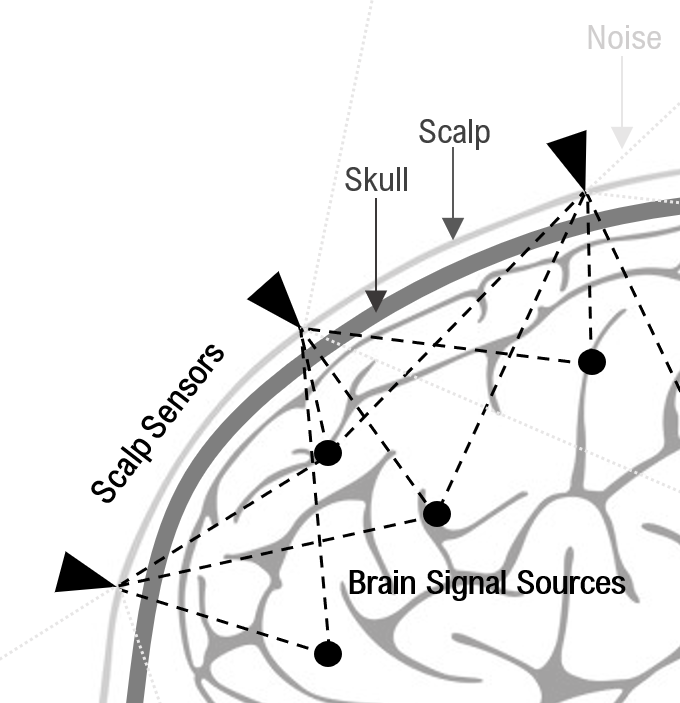
\includegraphics[width=\textwidth]{figures/EEG/volumeconduction.png}
        \caption{Illustration of volume conduction}\label{fig:volumeconduction}
    \end{minipage} 
    \hfill
    \begin{minipage}[t]{.45\textwidth}
        \centering
        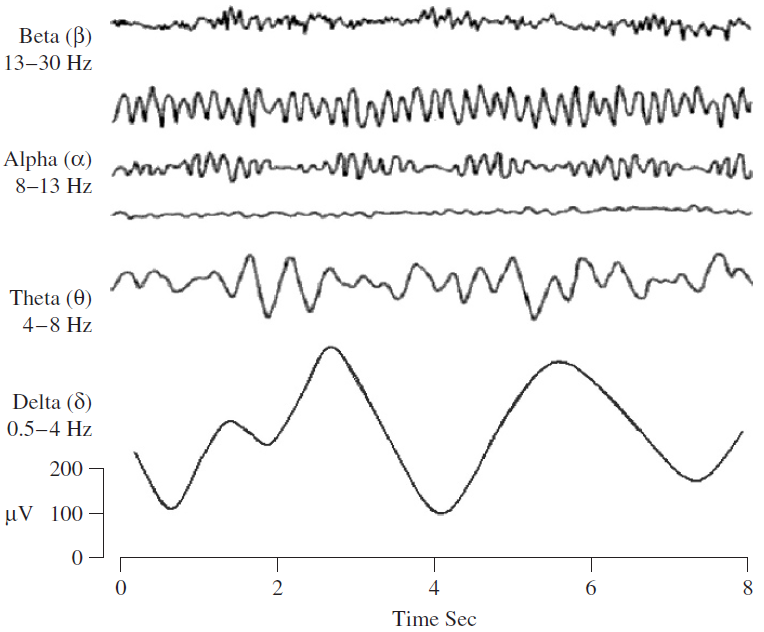
\includegraphics[width=\textwidth]{figures/EEG/EEG_example.png}
        \caption{Example of time dependent EEG measurements within the four defined categories, source: \cite{EEGsignalprocessing}}\label{fig:EEG_example}
    \end{minipage}
\end{figure}

\subsection{Application}\label{seg:application}
EEG performed on humans and animals have a great number of applications with both clinical and research purposes. 
Examples of clinical applications covers diagnosis and management of neurological disorders such as epilepsy and monitor alertness regarding coma or brain death.
EEG capitalizes on the procedure being non-invasive and fast.
Neural activity can be measured within fractions of a second after a stimuli has been provided. 
These advantages contributes to the wide range of applications within research of the neural processes involved in or resulting from actions, emotions or  cognition. Today such neural research are use in many different fields \cite[p. 4]{fundamentalEEG}.
% such as neuromarketing, biofeedback(optimisation of learning) and brain computer interface.  
The hearing aid industry is one example where this research is highly prioritized. 
At Eriksholm research center, which is a part of the hearing aid manufacturer Oticon, cognitive hearing science is a research area within fast development \cite{Weberik}. 
One main purpose at Eriksholm is to make it possible for a hearing aid to identify the user-intended sound source from real time EEG measurements and thereby exclude noise from elsewhere \cite{Emina2019} \cite{Bech2018}. 
It is essentially the well known but unsolved cocktail problem which is sought improved by use of EEG. 
This is where EEG and occasionally so called in-ear EEG is interesting. In conjunction with the technology of beamforming it is possible for a hearing aid to receive only signals from a specific direction. 

Over the past two decades, functional integration has become an area of interest regarding EEG research \cite{Friston2011}. 
Within neurobiology functional integration refers to the study of the correlation among activities in different regions of the brain. 
In other words, how do different parts of the brain work together to process information and conduct a response \cite{Friston2002}.     
For this purpose separation and localization of the original sources which contribute to the EEG measurement is of interest. 
An article from 2016 \cite{Van2019} points out the importance of performing analysis regarding functional integration at source level rather than at EEG level. 
It is argued through experiments that analysis at EEG level does not allow interpretations about the interaction between sources. 
This emphasize a potential for improving results within a wide range of EEG research, if the original active sources can be extracted from a specific EEG measurements.    

%     
%However, the focus of this research is the correlation between EEG measurements and the sound source rather than localization of the activated source from the EEG \cite{Emina2019}. 
%Hence a source localization approach could potentially be of interest regarding hearing aids in order to improve the results.
%(Furthermore, a real-time application to provide feedback from EEG measurements would be essential.)\todo{?}. 


\subsection{Modelling}
Consider the issue of extracting the activated sources from  EEG measurements on the scalp. A known approach is to model the observed data by a linear system 
\begin{align*}
\mathbf{y} = \mathbf{Ax}.
\end{align*}
The vector $\mathbf{y} \in \mathbb{R}^{M}$ is the EEG measurement of one time sample containing $M$ sensor measurements. $\mathbf{x} \in \mathbb{R}^{N}$ is the corresponding $N$ sources within the brain. 
The non-zero entries of $\textbf{x}$ represent the active sources at the time of the measurement. 
$\mathbf{A} \in \mathbb{R}^{M \times N}$ is an unknown projection/transformation(?) matrix, also referred to as the mixing matrix resembling the volume conduction. 
The $i$-th column of $\mathbf{A}$ represents the relative projection weights from the $i$-th source to every sensor \cite{phd2015}. 
Representing one time sample the linear system is in general referred to as a single measurement vector model. 
It it only the measurement vector $\textbf{y}$ that is known hence it is not possible to solve the linear system with respect to $\textbf{x}$ using basic linear algebra.   
The task in this case is to identify both $\mathbf{A}$ and then $\mathbf{x}$, given the measurement vector $\mathbf{y}$. This problem is referred to as the inverse problem of EEG. 
Finding $\textbf{x}$ from the inverse problem is referred to as source separation and localization. Separation is to find the signal of each active source and localization is to place each active source signal at the right position within the source vector of dimension $N$, where $N$ is the maximum number of sources to be active \todo{der er vel ikke N aktive source her?}.      
\subsection{Solution Method}\label{sec:ICAsolution}
Independent Component Analysis (ICA) is one commonly applied method to solve the inverse problem of EEG \cite{Scott1996}, \cite{Scott1997}. ICA is a technique to find the matrix $\mathbf{A}$ such that the column wise elements of $\mathbf{X}$ is statistically independent. Thus statistical independence between the active sources is the essential assumption, which in the case of EEG are considered valid due to the volume conduction being effectively instantaneous \cite[p. 3]{Scott1997}. 
Application of ICA has shown great results regarding source separation of high-density EEG. 
However, a significant flaw to this method is that the EEG measurements are only separated into a number of sources that is equal to or less than the number of sensors \cite{Balkan2015}.
Meaning that the EEG inverse problem can not be solved when  it forms an under-determined system, which is the case when the maximum number of unknown sources $N$ exceeds the number of sensors $M$. 
Such assumption undermines the reliability and usability of ICA, as the number of active sources easily exceed the number of sensors \cite{phd2015}. 
This is especially a drawback when low-density EEG are considered. Low-density EEG measurements are collected from equipment with less than 32 sensors, increasing the changes of $M$ being less that $N$. 
However, improved capabilities of low-density EEG devices are desirable due to their relative low cost, mobility and ease to use. 

This argues the importance of considering the inverse problem of EEG in the under-determined case where $N>M$. In the next section existing work considering the under-determined inverse problem of EEG is investigated further. 

\section{Related Work and Our Objective}\label{sec:relatedwork}
As mentioned above ICA is a solid method for source separation in the case where separation into a number of sources equal to the number of sensors is adequate. The issue occurs in cases where the number of sources $N$ exceeds the number of sensors $M$.  
To overcome this issue an extension of ICA was suggested, referred to as the ICA mixture model \cite{Balkan2015}.
Instead of identifying one overcomplete mixing matrix $\mathbf{A} \in \mathbb{R}^{M \times N}$ this approach learns $N_{\text{model}}$ different mixing matrices $\mathbf{A}_i \in \mathbb{R}^{M\times M}$, to make computations more tractable. 
This method was further adapted into the Adaptive Mixture ICA (AMICA) which showed successful results regarding identification of more sources than sensors \cite{Palmer2008}. 
However, these successful results relies on the assumption that no more than $M$ out of $N$ possible sources is simultaneously active. That is explicit that the source vector of dimension $N$ has at most $M$ non-zero entries.
This assumption is still an essential limitation to the frame work, especially when considering low-density EEG. 
Other types of ICA algorithms for under-determined systems have been proposed, without overcoming the limitation of jointly active sources exceeding the number of sensors.
%One is the Restricted ICA (RICA), an efficient method used for unsupervised learning in neural networks \cite{Le2011}.\\ 

In 2015 O. Balkan et. al. suggested a new approach also targeting the identification of more active sources than sensors regarding EEG measurements. One method is proposed for learning $\textbf{A}$ from $\textbf{y}$ \cite{Balkan2015} and a different method is proposed for finding $\textbf{x}$ given $\textbf{y}$ and $\textbf{A}$ \cite{Balkan2014}.

To learn $\textbf{A}$ the suggested method, referred to as Cov-DL, is a covariance-domain based dictionary learning algorithm. 
The method is based upon theory of dictionary learning and compressive sensing. Which dictates a framework for solving an under-determined system when $\textbf{x}$ contains a sufficiently amount of zeros. 
This is similar to the constraint of ICA.  However, to overcome this the point is to transfer the EEG measurements into the covariance domain. In the covariance domain a higher dimensionality can be achieved compared to the original EEG sensor domain with dimension $M$.
The transformation can be done when assuming a linear volume conduction and uncorrelated sources.
As a result the theory of compressive sensing is found to  apply to the covariance domain, allowing to learn $\textbf{A}$ by dictionary learning -- even in the case where the active sources exceeds the number of measurements.

The Cov-DL algorithm stands out from other straight forward dictionary learning methods as it does not relay on the sparsity of active sources\todo{is it okay to mention sparsity here for the first time?}. This is an essential advantage when low-density EEG is considered. 
Cov-DL was tested and found to outperform AMICA \cite{Balkan2015}.  
As mentioned, the Cov-DL algorithm only learns the mixing matrix $\mathbf{A}$, resembling the volume conduction.

For the purpose of recovering $\textbf{x}$, from $\textbf{y}$ and $\textbf{A}$, a multiple measurement sparse Bayesian learning (M-SBL) algorithm is proposed. This method is also targeting the case of more active sources than sensors.\todo{yderligere beskrivelse nødvedig? eller fjerne lidt fra Cov måske, da det samme lidt kommer i kap 3?}
The method was proven to outperform the previously used algorithms, even when the defined recovery conditions regarding the found mixing matrix $\textbf{A}$ was not fulfilled \cite{Balkan2014}.

One drawback, which is not fully covered in the referred literature, is that the two methods rely on the number of active sources being known. 
In practise this is not the case. 
Hence an estimation of the number of active sources has to be considered for the algorithm to be useful in practice. To address this issue a simple approach is to optimise the result with respect to the number active source, provided that some prior assumption of the expected result can be made.      
\\ \\
The two state of the art methods resulting in source separation and localization will make the foundation of this thesis. 
Our aim is to investigate and fully understand the two methods in order to implement and test a joint algorithm -- recovering the original sources $\textbf{x}$ from the measurements $\textbf{y}$, when the number of active sources exceeds the number of measurements. 
Secondary it is of interest to consider the practical application of the algorithm, for instance within a hearing aid as described in section \ref{sec:EEG}.  
%As described in section \ref{sec:EEG}  it is of interest to reduce the amount of energy it takes to listen to a specific sound source surrounded by noise.
%For this purpose we want to relate the found number of active sources to the level of concentration that the test person is experiencing. 
As mentioned, the number of active sources is in general unknown in practise thus it is first of all an estimation of the number of active sources which is of interest for practical use of the algorithm. 
For this we want to investigate whether it is possible to estimate the number of active sources, through optimization.   
 


 

\chapter{Problem Statement}\label{ch:problemstatement}
Through chapter \ref{ch:motivation} the potential of EEG measurement and especially low-density EEG measurements have been established. Furthermore, this potential is found to be increased through recovery of the original brain sources given the measurements. This involves solving the EEG inverse problem, in the case of the problem being under-determined.
Two state of the art methods are seen to solve the issue with success, but the use of a parameter unknown in practise limits the potential of the methods for practical use.

This motivates the following problem statement.         
\\ \\
\textit{Based on state of the art methods, how can the original sources of brain activity be recovered from the EEG inverse problem, in the under-determined case, and how can this be modified to increase the potential of practical use?}
\\ \\
From the problem statement the following sub-questions is established for clarification.
\begin{itemize}
\item How can Cov-DL be used to estimate the mixing matrix $\mathbf{A}$ from the overcomplete EEG inverse problem?
\item How can M-SBL be used to estimate the source matrix $\mathbf{X}$ from the overcomplete EEG inverse problem?
\item How can the above methods be implemented as one application performing source recovery from EEG measurements in real-time? 
\item How can the number of active sources be estimated, based only on the EEG measurement? 
\end{itemize}
\todo{is og have}

 
%\chapter{Sparse Signal Recovery}
This chapter gives an introduction to the concept compressive sensing. Associated theory regarding sparse signal recovery is described along the limitations of the common solution approaches. Finally the state of the art methods regarding non-sparse signal is presented. 
    
\section{Linear Algebra}
Some measurement vector $\mathbf{y}$ can be described as a linear combinations of a coefficient matrix $\mathbf{A}$ and some vector $\mathbf{x}$ such that
\begin{align}\label{eq:SMV_model}
\mathbf{y} &= \mathbf{Ax},
\end{align}
where $\mathbf{y} \in \mathbb{R}^M$ is the observed measurement vector consisting of $M$ measurements, $\mathbf{x} \in \mathbb{R}^N$ is an unknown vector of $N$ elements, and $\mathbf{A} \in \mathbb{R}^{M \times N}$ is a coefficient matrix which models the linear measurement process column-wise. The liner model makes a system of linear equations with $M$ equations and $N$ unknowns.
\\ \\
In the case of $\mathbf{A}$ being a square matrix, $M = N$, a solution can be found to the linear model if $\mathbf{A}$ has full rank -- $\mathbf{A}$ consist of linearly independent columns or rows.
% For $M > N$ the matrix said to have full rank when the columns are linearly independent. For $M < N$ the matrix has full rank when the rows are linearly independent. 
A linear systems with $M = N$ is called determined, $M > N$ overdetermined and $M < N$ under-determined. 
When full rank do not occur the matrix is then called rank-deficient.
\\ \\
By inverting $\mathbf{A}$ from \eqref{eq:SMV_model} the unknown vector $\mathbf{x}$ can be achieved. Square matrix is invertible if an only if its has full rank or its determinant $\det(\mathbf{A}) \neq 0$. For rectangular matrices, $M > N$ and $M < N$, left-sided and right-sided inverse exists.
%\begin{itemize}
%\item Left-sided inverse ($M > N$): $(\mathbf{A} \mathbf{A})^{-1} \mathbf{A}^T \mathbf{A} = \mathbf{A}_{\text{left}}^{-1} = \mathbf{I}_N$ 
%\item Right-sided inverse ($M < N$): $\mathbf{A} \mathbf{A}^T (\mathbf{A} \mathbf{A}^T)^{-1} = \mathbf{A}_{\text{right}}^{-1} = \mathbf{I}_M$ 
%\end{itemize}
With the left-inverse the least norm solution of \eqref{eq:SMV_model} can be found.\todo{least norm solution?}
\\ \\
For an determined system there will exist a unique solution. For an overdetermined system there do not exist a solution and for under-determined systems there exist infinitely many solutions\cite[p. ix]{CS}.
\\ 
As described in chapter \ref{ch:motivation} the linear model of interest consist of $M$ sensors which makes the observed measurements $\textbf{y}$ and $N$ sources which makes the unknown vector $\textbf{x}$. Here it is of interest to find a solution to the case where the system consist of more sources than sensors -- hence a solution has to be found within the infinitely solution set.

\section{Compressive Sensing}\label{sec:CS}
Compressive sensing is the theory of efficient recovery or reconstruction of a signal from a minimal number of observed measurements. It is build upon empirical observations assuring that many signals can be approximated by remarkably sparser signals.   
 Assume linear acquisition of the original measurements, then the relation between the measurements and the signal to be recovered can be described by the linear model \eqref{eq:SMV_model} \cite{FR}.  
\\ 
%\begin{align}\label{eq:model}
%\mathbf{y} = \mathbf{Ax}.
%\end{align}
%Here $\mathbf{y} \in \mathbb{R}^M$ is the measured data consisting of $M$ observations, $\mathbf{x} \in \mathbb{R}^N$ is the original signal consisting of $N$ possible sources. $\mathbf{A} \in \mathbb{R}^{M \times N}$ is a matrix which models the linear measurement process or in other words it projects each of the $N$ possible sources on to the $M$ observations. $\textbf{A}$ is  referred to as a dictionary or a mixing matrix .\\
In compressive sensing terminology, $\mathbf{x}\in \mathbb{R}^{N}$ is the signal of interest which is sought recovered from the measurements $\textbf{y}\in \mathbb{R}^{M}$ by solving the linear system \eqref{eq:SMV_model}. The coefficient matrix $\textbf{A}$ is in the context of compressive sensing referred to as the mixing matrix or the dictionary matrix.\\    
 In the typical compressive sensing case the system is under-determined, $M < N$,  and there exist infinitely many solutions, provided that a solution exist.
% Such system is also referred to as over-complete \textit{(as the number of column basis vectors is greater than the dimension of the input)}.
\\
However, by enforcing certain sparsity constraints it is possible to recover the wanted signal, hence the term sparse signal recovery \cite{FR}.
%Yet another argument; If $M<<N$, it leads to the matrix $\mathbf{A}$ being rank-deficient\textit{(but not necessarily?)} which imply that $\mathbf{A}$ has a non-empty null space and this leads to infinitely many signals which yield the same solution $\mathbf{y} = \mathbf{Ax} = \mathbf{Ax'}$ \cite[p. ix]{CS}. Thus it is necessary to limit the solution space to a specific class of signals $\mathbf{x}$, for this a certain constraint on sparseness is introduced.   

\subsection{Sparseness} 
A signal is said to be $k$-sparse if the signal has at most $k$ non-zero coefficients. For the purpose of counting the non-zero entries of a vector representing a signal the $\ell_0$-norm is defined
\begin{align*}
\Vert \mathbf{x} \Vert_0 := \text{card}(\text{supp}(\mathbf{x})).
\end{align*}
The function $\text{card}(\cdot)$ gives the cardinality of the input and the support vector of $\mathbf{x}$ is given as
\begin{align*}
\text{supp}(\mathbf{x}) = \{ j \in [N] \ : \ x_j \neq 0 \},
\end{align*} 
where $[N]$ is a set of integers $\{1,2,\hdots,N\}$ \cite[p. 41]{FR}. The set of all $k$-sparse signals is denoted as
\begin{align*}
\Omega_k = \{ \mathbf{x} \ : \ \Vert \mathbf{x} \Vert_0 \leq k \}.
\end{align*}

\subsection{Optimisation Problem}\label{sec:opti}
To find a solution to the linear model \eqref{eq:SMV_model} assuming the solution is $k$-sparse, it can be view as an optimisation problem. An optimisation problem is defined as
\begin{align*}
\min f_0 (\mathbf{x}) \quad \text{s.t} \quad f_i (\mathbf{x}) \leq b_i, \quad i = 1,2, \hdots, n ,
\end{align*}
where $f_0 \ : \ \mathbb{R}^N \mapsto \mathbb{R}$ is an objective function and $f_i \ : \ \mathbb{R}^N \mapsto \mathbb{R}$ are the constraint functions. 
\\
To find the $k$-sparse solution our optimisation problem can be written as
\begin{align*}
\textbf{x}^\ast = \arg \min_{\textbf{x}\in \boldsymbol{\Omega_{k}}} \Vert \mathbf{x} \Vert_0 \quad \text{s.t} \quad \mathbf{y} = \mathbf{Ax},
\end{align*}
The objective function is given by an $\ell_0$ norm with the constraint function being the linear model \eqref{eq:SMV_model}. Unfortunately, this optimisation problem is non-convex due to the definition of $\ell_0$-norm and is therefore difficult to solve -- it is a NP-hard problem. Instead, by replacing the $\ell_0$-norm with the $\ell_1$-norm, the optimisation problem can be approximated and hence become computational feasible\todo{skal vi indføre z som en approx af x, også et nyt omega eller? eller kan vi beholde x} \cite[p. 27]{CS}
\begin{align}\label{eq:SMV_p1}
\textbf{x}^\ast = \arg \min_{\textbf{x}\in  \boldsymbol{\Omega_{k}}} \Vert \mathbf{x} \Vert_1 \quad \text{s.t} \quad \mathbf{y} = \mathbf{Ax}.
\end{align} 
With this optimisation problem we find the best $k$-sparse solution $\mathbf{x}^\ast$. This method is referred to as Basis Pursuit. 
\\
The following theorem justifies that the $\ell_1$ optimisation problem finds a sparse solution \cite[p. 62-63]{FR}.
\begin{theorem}
A mixing matrix $\mathbf{A} \in \mathbb{R}^{M \times N}$ is defined with columns $\textbf{A} = [\textbf{a}_1, \dots, \textbf{a}_N]$. By assuming uniqueness of a solution $\textbf{x}^{\ast}$ to
$$
\min_{\textbf{x} \in \mathbb{R}^N} \Vert \textbf{x} \Vert_1 \quad \text{s.t} \quad \textbf{Ax} = \textbf{y},
$$
the system $\{ \textbf{a}_j, j \in \text{supp} ( \textbf{x}^{\ast})\}$ is linearly independent, and in particular
$$
\Vert \textbf{x}^{\ast} \Vert_0 = \text{card}(\text{supp} (\textbf{x}^{\ast})) \leq M.
$$
\end{theorem}
To prove this theorem we need to realise that the set $\{\textbf{a}_j, j \in S \} \leq M$, with $S = \text{supp}(\textbf{x}^\ast)$, can not have more than $M$ linearly independence columns. So when $M \ll N$ we automatically achieve a sparse signal.
\begin{proof}
For the case of contradiction, assume that the set $\{\textbf{a}_j, j \in S \}$ is linearly dependent. Thus there exists a non-zero vector $\textbf{v} \in \mathbb{R}^N$ supported on $S$ such that $\textbf{Av} = \textbf{0}$. Then, for any $t \neq 0$,
$$
\Vert \textbf{x}^{\ast} \Vert_1 < \Vert \textbf{x}^{\ast} + t \textbf{v} \Vert_1 = \sum_{j \in S} \vert x_j^{\ast} + t v_j \vert = \sum_{j \in S} \text{sgn}(x_j^{\ast} + t v_j )(x_j^{\ast} + t v_j ).
$$
If $|t|$ is small enough, namely, $|t| < \min_{j \in S} \vert x_j^{\ast}\vert / \Vert \textbf{v} \Vert_{\infty}$, then
$$
\text{sgn}(x_j^{\ast} + t v_j) = \text{sgn}(x_j^{\ast}), \quad \forall j \in S.
$$
It the follows that
$$
\Vert \textbf{x}^{\ast} \Vert_1 < \sum_{j \in S} \text{sgn}(x_j^{\ast})(x_j^{\ast} + t v_j ) = \sum_{j \in S} \text{sgn}(x_j^{\ast})x_j^{\ast} + t \sum_{j \in S} \text{sgn}(x_j^{\ast})v_j = \Vert \textbf{x}^{\ast} \Vert_1 + t \sum_{j \in S} \text{sgn}(x_j^{\ast})v_j.
$$
This is a contradiction, because we can always choose a small $t \neq 0$ such that $t \sum_{j \in S} \text{sgn}(x_j^{\ast})v_j \leq 0$ and therefore the set $\{\textbf{a}_j, j \in S \}$ must be linearly independent\todo{kan vi lige gennemgå dette. }.
\end{proof}
The Basis Pursuit makes the foundation of several algorithms solving alternative versions of \eqref{eq:SMV_p1} where noise is incorporated. An alternative solution method includes greedy algorithms such as the Orthogonal Matching Pursuit(OMP) \cite[P. 65]{FR}. At each iteration of the OMP algorithm an index set $S$ is updated by adding the index corresponding to the column in $\textbf{A}$ that best describes the residual, hence greedy. That is the part of $\textbf{y}$ that is not yet explained by $\textbf{Ax}$ is included. Then $\textbf{x}$ is updated as the vector, supported by $S$, which minimize the residual, that is also the orthogonal projection  of $\textbf{y}$ onto the span$\{a_j \ \vert \ j \in S \}$. 
\begin{algorithm}[H]
\caption{Orthogonal Matching Pursuit (OMP)}
\begin{algorithmic}[1]
			\State$k = 0$			
			\State$\text{Initialize} \quad S_{(0)} =\emptyset$ 
			\State$\text{Initialize} \quad x_{(0)} =\textbf{0}$
            \Procedure{OMP}{$\textbf{A},\textbf{y}$}    
            \While{$\text{stopping criteria not meet}$} 
                \State$k = k + 1$
				\State$j_{(k)} = \arg \max_{j \in [N]} \{ \vert (\mathbf{A}^\ast (\mathbf{y} - \mathbf{Ax}_{(k-1)}))_j\vert \}$				
				\State$S_{(k)} = S_{(k-1)} \cup \lbrace j_{(k)} \rbrace$ 
				\State$\textbf{x}_{(k)} = \arg \min_{\mathbf{z} \in \mathbb{C}^N} \{ \Vert \mathbf{y} - \mathbf{Az} \Vert_2 \  \vert \ \text{supp}(\mathbf{z}) \subset S_{(k)} \}$
          		\EndWhile
          		\State$\mathbf{x}^\ast = \mathbf{x}_{(k)}$
            \EndProcedure
        \end{algorithmic} 
        \label{alg:OMP}
\end{algorithm}


      
\subsection{Conditions on the Mixing Matrix}\label{sec:dic_conditions}
In section \ref{sec:opti} the mixing matrix $\mathbf{A}$ was assumed known, in order to solve the optimisation problem \eqref{eq:SMV_p1}. However, in practise it is only the measurement vector $\textbf{y}$ which is known. In this case the mixing matrix $\textbf{A}$ is considered a estimate of the true mixing matrix. In general compressive sensing terminology  $\textbf{A}$ is also referred to as a dictionary matrix.\\
To ensure exact or approximately reconstruction of the sparse signal $\mathbb{x}$, the mixing matrix must be constructed with certain conditions in mind. 
% $\mathbf{x}^\ast$ from the optimisation problem \eqref{eq:SMV_p1} 


\subsubsection{Null Space Condition}
The the null space property is a necessary and sufficient condition to $\mathbf{A}$ for exact reconstruction of every sparse signal $\textbf{x}$ that solves the optimisation problem \eqref{eq:SMV_p1}\cite[p. 77]{FR}. The null space of the matrix $A$ is defined as
\begin{align*}
\mathcal{N}(\mathbf{A}) = \{ \mathbf{z} \ : \ \mathbf{Az} = \textbf{0} \}.
\end{align*} 
The null space property is defined as
\begin{definition}[Null Space Property]
A matrix $\mathbf{A} \in \mathbb{R}^{M \times N}$ is said to satisfy the null space property relative to a set $S \subset [N]$ if
\begin{align}
\Vert \textbf{v}_S \Vert_1 < \Vert \textbf{v}_{\overline{S}} \Vert_1 \quad \text{for all} \quad \textbf{v} \in \text{null}(\mathbf{A} \setminus \lbrace \textbf{0} \rbrace),
\end{align}
where the vector $\mathbf{v}_S$ is the restriction of $\mathbf{v}$ to the indices in $S$, and $\bar{S}$ is the set $[N]\setminus S$. 
\end{definition}

\begin{theorem}
Given a matrix $\textbf{A} \in \mathbb{R}^{M \times N}$, every vector $\textbf{x} \in \mathbb{R}^N$ with $\text{supp}(\textbf{x})\subset S$ is the unique solution of \eqref{eq:SMV_p1} with $\textbf{y} = \textbf{Ax}$ if and only if $\textbf{A}$ satisfies the null space property relative to $S$.
\end{theorem}
\begin{proof}
$\Rightarrow:$  Let $S \subseteq [N]$ be a fixed index set. Assume that any vector $\textbf{x} \in \mathbb{R}^N$ with support $\text{supp}(\textbf{x})\subset S$ is the unique minimiser of $\Vert \textbf{z} \Vert_1$ with respect to $\textbf{Az} = \textbf{Ax}$. Thus, for any $\textbf{v} \in \text{null}(\mathbf{A}) \setminus \{\textbf{0} \}$, the vector $\textbf{v}_S$ is the unique minimizer $\Vert \textbf{z} \Vert_1$ the respect to $\textbf{Az} = \textbf{Av}_S$. But we have that $\textbf{0} = \textbf{A}(\textbf{v}_S + \textbf{v}_{\overline{S}}) \implies \textbf{Av}_S = \textbf{A}(-\textbf{v}_{\overline{S}})$ and $-\textbf{v}_{\overline{S}} \neq \textbf{v}_S$ or else $\textbf{v} = \textbf{0}$. We conclude that $\Vert \textbf{v}_S \Vert_1 < \Vert \textbf{v}_{\overline{S}} \Vert_1$. This establishes the null space property relative to $S$.
\\ \\
$\Leftarrow:$ Conversely, assume that the null space property relative to $S$ holds. Then, given $S \subseteq [N]$ with null space property and a vector $\textbf{x} \in \mathbb{R}^N$ with $\text{supp}(\textbf{x})\subset S$ and a vector $\textbf{z} \in \mathbb{R}^N$, $\textbf{z} \neq \textbf{x}$, such that $\textbf{Az} = \textbf{Ax}$, we consider the vector $\textbf{v} := \textbf{x} - \textbf{z} \in \text{null}(\textbf{A}) \setminus \{ \textbf{0} \}$. From the null space property, the following is obtained
\begin{align*}
\Vert \textbf{x} \Vert_1 \leq \Vert \textbf{x} - \textbf{z}_S \Vert_1 &= \Vert \textbf{v}_S \Vert_1 + \Vert \textbf{z}_S \Vert_1 \\
&< \Vert \textbf{v}_{\overline{S}} \Vert_1 + \Vert \textbf{z}_S \Vert_1 \\
&= \Vert -\textbf{z}_{\overline{S}} \Vert_1 + \Vert \textbf{z}_S \Vert_1 = \Vert \textbf{z} \Vert_1
\end{align*}
This establishes the required sparseness of $\Vert \textbf{x} \Vert_1$.
\end{proof}
Unfortunately, this is a condition which is hard to check in practice.

\subsubsection{Coherence}
The null space property provide a unique solution to the optimisation problem \eqref{eq:SMV_p1}, but it is unfortunately complicated to investigate. Instead an alternative measure is presented.
\\
Coherence is a measure of quality, it determines whether a matrix $\mathbf{A}$ is a good choice for the optimisation problem \eqref{eq:SMV_p1}. A small coherence describes the performance of a recovery algorithm as good with that choice of $\mathbf{A}$. 
\begin{definition}[Coherence]
Coherence of the matrix $A \in \mathbb{R}^{M \times N}$, denoted as $\mu (\mathbf{A})$, with columns $\mathbf{a}_1, \dots, \mathbf{a}_N$ for all $i \in [N]$ is given as
\begin{align*}
\mu (\mathbf{A}) = \max_{1 \leq i < j \leq n} \frac{\vert \langle a_i, a_j \rangle \vert}{\Vert a_i \Vert_2 \Vert a_j \Vert_2}.
\end{align*}
\end{definition}

\subsubsection{Restricted Isometry Condition}
Restricted isometry condition is a stronger condition concerning the orthogonality of the matrix $\mathbf{A}$.
\begin{definition}[Restricted Isometry Property]
A matrix $A$ satisfies the RIP of order $k$ if there exists a $\delta_k \in (0,1)$ such that
\begin{align*}
(1 - \delta_k) \Vert x \Vert_2^2 \leq \Vert Ax \Vert_2^2 \leq (1 + \delta_k) \Vert x \Vert_2^2,
\end{align*}%holds for all $x \in \Sigma_k$
\end{definition}

\begin{theorem}
Suppose that the $2s$-th restricted isometry constant of the matrix $\textbf{A} \in \mathbb{R}^{M \times N}$ satisfies
\begin{align*}
    \delta_{2s} < \frac{1}{3}.
\end{align*}
Then every $s$-sparse vector $\textbf{x}^\ast \in \mathbb{R}^N$ is the unique solution of
$$
\min_{\textbf{z} \in \mathbb{R}^N} \Vert \textbf{z} \Vert_1 \quad \text{subject to} \quad \textbf{Az} = \textbf{Ax}.
$$
\end{theorem}
\begin{proof}
To proof the theorem we only need to show the null space condition:
$$
\Vert \textbf{v} \Vert_1 < \frac{1}{2} \Vert \textbf{v} \Vert_1, \quad \forall \ \textbf{v} \in \text{ker}(\textbf{A})\setminus \{\textbf{0}\}, \ S \subseteq [N], \ \text{card}(S) \leq s.
$$
Cf. Cauchy-Schwarz or $\Vert \textbf{v}_S \Vert_1 \leq \Vert \textbf{v}_S \Vert_2 \sqrt{s}$, we only need to show
\begin{align*}
\Vert \textbf{v}_S \Vert_2 &\leq \frac{\rho}{2 \sqrt{s}} \Vert \textbf{v} \Vert_1 \\
\rho &= \dfrac{2 \delta_{2s}}{1 - \delta_{2s}} < 1,
\end{align*}
whenever $\delta_{2s} < 1/3$. Given $\textbf{v} \in$ ker$(\textbf{A})\setminus \{\textbf{0}\}$, it is enough to consider an index set $S = S_0$ of $s$ largest absolute entries of the vector $\textbf{v}$. The complement $\overline{S_0}$ of $S_0$ in $[N]$ is partition as $S_0 = S_1 \cup S_2 \cup \cdots$, where
\begin{align*}
    S_1 \ &: \ \text{index set of } s \text{ largest absolute entries of } \textbf{v} \text{ in } \overline{S_0}, \\
    S_2 \ &: \ \text{index set of } s \text{ largest absolute entries of } \textbf{v} \text{ in } \overline{S_0 \cup S_1}.
\end{align*}
With $\textbf{v} \in$ ker$(\textbf{A})$:
$$
\textbf{A}(\textbf{v}_{S_0}) = \textbf{A}(-\textbf{v}_{S_1} - \textbf{v}_{S_2} - \cdots),
$$
so that
\begin{align}\label{eq:L9_6}
\Vert \textbf{v}_{S_0} \Vert_2^2 &\leq \frac{1}{1 - \delta_{2s}} \Vert \textbf{A}(\textbf{v}_{S_0}) \Vert_2^2 = \frac{1}{1 - \delta_{2s}} \langle \textbf{A}(\textbf{v}_{S_0}), \textbf{A}(-\textbf{v}_{S_1}) + \textbf{A}(-\textbf{v}_{S_2}) + \cdots \rangle \nonumber \\
    &= \frac{1}{1 - \delta_{2s}} \sum_{k \geq 1} \langle \textbf{A}(\textbf{v}_{S_0}), \textbf{A}(-\textbf{v}_{S_k}) \rangle.
\end{align}
According to Proposition \ref{prop:L9_1}, we also have
\begin{align}\label{eq:L9_7}
    \langle \textbf{A}(\textbf{v}_{S_0}), \textbf{A}(-\textbf{v}_{S_k}) \rangle. \leq \delta_{2s} \Vert \textbf{v}_{S_0} \Vert_2 \Vert \textbf{v}_{S_k} \Vert_2.
\end{align}
Substituting \eqref{eq:L9_7} into \eqref{eq:L9_6} and dividing by $\Vert \textbf{v}_{S_0} \Vert_2 > 0$
\end{proof}

%The construction of the matrix $\mathbf{A}$ is of course essential for the solution of the optimisation problem. So far no one has manage to construct a matrix which is proved to be optimal for some compressive sensing set up. However some certain constructions have shown sufficient recovery guarantee.\\ \\
%To ensure an exact or an approximate reconstruction of the sparse signal $\mathbf{x}$ some conditions associated to the matrix $\mathbf{A}$ must be satisfied.\\
%This includes at first the null space condition, a property of the $A$ matrix which is hard to check in practise. 
%The Restricted isometry condition is a stronger condition concerning the orthogonality of the matrix. Furthermore the coherence of a matrix is a measure of quality and is used to determine whether the matrix $A$ is a good choice for the optimisation problem.\\    

\subsection{Multiple Measurement Vector Model}\label{sec:MMV}
The linear model \eqref{eq:SMV_model} is also referred to as a single measurement vector (SMV) model. In order to adapt the model \eqref{eq:SMV_model} to a practical use the model is expanded to include multiple measurement vectors and take noise into account.
\\ \\
A multiple measurement vector (MMV) model consist of the observed measurement matrix $\mathbf{Y} \in \mathbb{R}^{M \times L}$, the source matrix $\mathbf{X} \in \mathbb{R}^{N \times L}$, the dictionary matrix $\mathbf{A} \in \mathbb{R}^{M \times N}$ and the noise vector $\textbf{E} \in \mathbb{R}^{M \times L}$:
\begin{align}\label{eq:MMV_model}
\mathbf{Y} = \mathbf{AX}+\textbf{E}.
\end{align}
$L$ denote the number of observed measurement vectors each consisting of $M$ measurements, that is $L$ samples is given. For $L = 1$ the linear model will just be the SMV model \eqref{eq:SMV_model}. 
\\
The matrix $\mathbf{X}$ consist of $\lbrace \mathbf{x}_i \rbrace_{i=1}^L$ $k$-sparse vectors which has been stacked column-wise such that $\mathbf{X}$ consist of at most $k$ non-zero rows\todo{vi skal lige have styr på om vi kun antager identisk sparsness i alle søjler, og i så fald at det data vi arbejde med har den form}. As for the SMV model \eqref{eq:SMV_model} the MMV model \eqref{eq:MMV_model} is under-determined with $M \ll N$ and $k < M$\cite[p. 42]{CS}.
\\ \\
The support of $\mathbf{X}$ denote the index set of non-zero rows of $\mathbf{X}$ and $\mathbf{X}$ is said to be row-sparse. As the columns in $\mathbf{X}$ are $k$-sparse and as mention before $\mathbf{X}$ has at most $k$ non-zero rows, the non-zero values occur in common location for all columns. By using this joint information it is possible to recover $\mathbf{X}$ from fewer measurements.
\\
By using the rank of $\mathbf{X}$, which give us information of the amount of linearly independent rows or columns, and the spark of $\mathbf{A}$ which is the minimum set of linearly dependent columns, it is possible to set some conditions on the system to ensure recovery.
\\
When $\vert \text{supp}(\mathbf{X})\vert = k$ then $\text{rank}(\mathbf{X}) \leq k$. If rank$(\mathbf{X}) = 1$ then are the $k$-sparse vectors $\lbrace \mathbf{x}_i \rbrace_{i=1}^L$ multiples of each other and the joint information can not be taken advantage of. But for large rank it is possible to exploit the diversity of the columns in $\mathbf{X}$. This can be defined as a sufficient and necessary condition of the MMV model \eqref{eq:MMV_model}. MMV system $\textbf{Y}=\textbf{AX}$ must have
\begin{align*}
\vert \text{supp}(\mathbf{X}) \vert < \frac{\text{Spark} (\mathbf{A}) - 1 + \text{rank}(\mathbf{X})}{2}
\end{align*}
such that $\mathbf{X}$ can uniquely be determined.
\\
This result says that a row-sparse matrix $\mathbf{X}$ with large rank can be recovered from fewer\todo{"fewer" skal lige præsiseres, evt. bare M measurements?} measurement \cite[p. 43]{CS}.

%\subsection{Dictionary learning}\label{sec:dictionarylearning}
%In cases where the dictionary is unknown it is possible to learn the dictionary from the observed measurement provided that several observations are available $\textbf{Y}=\left[ \textbf{y}_1, \dots ,\textbf{y}_L \right]$. 
%In dictionary learning framework the inverse problem is defined as
%\begin{align*}
%\min_{\mathbf{A,X}} = \frac{1}{2} \sum_{i=1}^{L} \Vert \mathbf{y} _i - \mathbf{Ax}_i \Vert_F^2 + \gamma \sum_{i=1}^{L} g(\mathbf{x}_i),
%\end{align*}
%where the function $g(\cdot)$ promotes sparsity of the source vectors at sample $i$ \cite[p. 4]{phd}. $\Vert \cdot \Vert_F$ is the Frobenius norm which is a vector norm defined as 
%\begin{align*}
%\Vert \mathbf{A} \Vert_F = \sqrt{\sum_{i=1}^M \sum_{j=1}^N \vert a_{i,j} \vert^2}.
%\end{align*}
%With the MMV model defined as a optimisation problem different dictionary learning algorithm can be used to learn the dictionary $\mathbf{A}$. One of them is the K-SVD algorithm.

\section{Dictionary learning}\label{sec:dictionarylearning}
As clarified in section \ref{sec:dic_conditions} the estimation of dictionary matrix $\textbf{A}$ is essential to achieve the best recovery of the sparse signal $\textbf{x}$ from the measurements $\textbf{y}$. Pre-constructed dictionaries do exist which in many cases results in simple and fast algorithms for reconstruction of $\textbf{x}$\cite{Elad_book}. Pre-constructed dictionaries are typically fitted to a specific kind of data, for instance the discrete Fourier transform or the discrete wavelet transform are used especially for sparse representation of images\cite{Elad_book}. Hence the results of using such dictionaries depend on how well they fit the data of interest, which is creating a certain limitation. An alternative is to consider an adaptive dictionary based on a set of training data that resembles the data of interest. For this purpose learning methods are considered to empirically construct a fixed dictionary which can take part in the application. Different dictionary learning algorithms exist, one is the K-SVD which is to be elaborated in this section. The K-SVD algorithm was presented in 2006 by Elad et al. and found to outperform pre-constructed dictionaries when computational cost is of secondary interest\cite{Elad2006}. \\
\\
Consider now $\textbf{Y}=\left[ \textbf{y}_1, \dots ,\textbf{y}_L \right]$, $\textbf{y}_i\in \mathbb{R}^{M}$ as a training database, created by $\textbf{y}_i=\textbf{A}\textbf{x}_i$ for which we want to learn the best suitable dictionary $\textbf{A}$ and sparse representation $\textbf{X}=\left[ \textbf{x}_1, \dots ,\textbf{x}_L \right]$, $\textbf{x}_i\in \mathbb{R}^{N}$. For a known sparsity constraint $k$ this can be defined by an optimisation problem similar to the general compressive sensing problem of multiple measurements \cite{Elad_book}
\begin{align}
\min_{\mathbf{A,X}} \sum_{i=1}^{L} \Vert \mathbf{y} _i - \mathbf{Ax}_i \Vert_2^2 \quad st. \ \Vert \textbf{x}_i\Vert_0\leq k, \ 1\leq i \leq L.\label{eq:SVD1}
\end{align}  
The learning consist of jointly solving the optimization problem on $\textbf{X}$ and $\textbf{A}$. The uniqueness of $\textbf{A}$ depends on the recovery sparsity condition. As clarified earlier recovery is only possible if $k < M$\cite{phd2015}. Furthermore, consider $\textbf{A}_0$ such that every training signal can be represented by $k_0 < \text{spark}(\textbf{A}_0)/2$ columns of $\textbf{A}_0$, then $\textbf{A}_0$ is a unique dictionary, up to scaling and permutation of columns\cite{Elad_book}\todo{fungerer disse to uniqueness parameter sammen?}. Again the $\ell_0$-norm lead to an NP-hard problem an heuristic methods are need.     

\subsection{K-SVD}
The dictionary learning algorithm K-SVD provide an update rule which is applied to each column of $\textbf{A}_0 = \left[ \textbf{a}_0, \hdots , \textbf{a}_N \right] $. Updating first $\textbf{a}_i$ and then the corresponding coefficients in $\textbf{X}$ which it is multiplied with, that is the $i^{\text{th}}$ row in $\textbf{X}$ denoted by $\textbf{x}_i^T$.\\
Let $\textbf{a}_{i_{0}}$ be the column to be updated and let the remaining columns be fixed. By rewriting the objective function in \eqref{eq:SVD1} using matrix notation it is possible to isolate the contribution from $\textbf{a}_{i_{0}}$.
\begin{align}
\Vert \textbf{Y} - \textbf{AX} \Vert_{F}^{2} 
&= \left\| \textbf{Y} - \sum_{i=1}^{M} \textbf{a}_i \textbf{x}_i^{T} \right\|_{F}^{2}\nonumber\\
&= \left\| \left( \textbf{Y}- \sum_{i\neq i_{i}}^{M} \textbf{a}_i\textbf{x}_i^{T}\right) - \textbf{a}_{i_{0}}\textbf{x}_{i_{0}}^{T} \right\| _{F}^{2},\label{eq:SVD2} 
\end{align}
where $F$ is the Frobenius norm that works on matrices
\begin{align*}
\Vert \mathbf{A} \Vert_F = \sqrt{\sum_{i=1}^M \sum_{j=1}^N \vert a_{i,j} \vert^2}.
\end{align*} 
In \eqref{eq:SVD2} the term in the parenthesis makes the an error matrix $\textbf{E}_{i_0}$ without the contribution from $i_{0}$, hence minimising \eqref{eq:SVD2} with respect to $\textbf{a}_{i_{0}}$ and $\textbf{x}_{i_{0}}^{T}$ leads to the optimal contribution from $i_{0}$ (can I say it this way..?). 
\begin{align}
\min_{\textbf{a}_{i_{0}},\textbf{x}_{i_0}^{T}}\left\|\textbf{ E}_{i_{0}}-\textbf{a}_{i_{0}},\textbf{x}_{i_0}^{T} \right\|_{F}^{2}\label{eq:SVD3}
\end{align} 
The optimal solution to \eqref{eq:SVD3} is known to be the rank-1 approximation of $\textbf{E}_{i_{0}}$. This comes from the Eckart–Young–Mirsky theorem\cite{?} saying that a partial single value decomposition(SVD) makes the best low-rank approximation of a matrix such as $\textbf{E}_{i_0}$.\\
That is specifically that for $\textbf{E}_{i_0}=\textbf{U}\boldsymbol{\Sigma}\textbf{V}^T\in \mathbb{R}^{M\times N},\ M \leq N$ with 
\begin{align*}
\textbf{U}=\left[\textbf{u}_1, \hdots, \textbf{u}_M\right] \in \mathbb{R}^{M\times M}, \quad \boldsymbol{\Sigma}=\text{diag}\left[\sigma_1, \hdots , \sigma_m \right] \in \mathbb{R}^{M\times N}, \quad \textbf{V}=\left[\textbf{v}_1, \hdots, \textbf{v}_N\right] \in \mathbb{R}^{N\times N} 
\end{align*}  
where $\textbf{U}$ and $\textbf{V}$ are unitary matrices, i.e. $\textbf{U}^T\textbf{U}=\textbf{UU}^T=\textbf{I}$, and $\sigma_j$ is the non-negative singular values of $\textbf{E}_{i_0}$ such that $\sigma_1\geq \sigma_2 \geq \hdots \geq 0$. The best $k$-rank approximation to $\textbf{E}_{i_0}$, with $k< rank(\textbf{E}_{i_0})$ is then given \todo{find kilde}by\cite{Wiki..} 
\begin{align*}
\textbf{E}_{i_{0}}^{(k)}= \sum_{j=1}^{k}\sigma_j\textbf{u}_{j}\textbf{v}_{j}^T.
\end{align*} 
Since the outer product always have rank-1 letting $\textbf{a}_{i_0}=\textbf{u}_1$ and $\textbf{x}_{i_0}^T = \sigma_{i}\textbf{v}_{1}^T$ solves the optimisation problem \eqref{eq:SVD3}.
However in order to preserve the sparsity in $\textbf{X}$ while optimising, only the non-zero entries in $\textbf{x}_{i_0}^T$ are allowed to vary. For this purpose only a subset of columns in $\textbf{E}_{i_0}$ is considered, those which correspond to the non-zero entries of $\textbf{x}_{i_0}^T$. A matrix $\textbf{P}_{i_0}$ is defined such that $\textbf{x}_{i_0}^{T^{(R)}}=\textbf{x}_{i_0}^T\textbf{P}_{i_0} $ is restricted to contain only the $M_{j_0}$ non-zero entries of $\textbf{x}_{i_0}^T$. By applying SVD to the  sub-matrix $\textbf{E}_{i_0}\textbf{P}_{i_0}$ and updating $\textbf{a}_{i_0}$ and $\textbf{x}_{i_0}^{T^{(R)}}$ the rank-1 approximation is found and the original representation vector is updated as $\textbf{x}_{i_0}^{T}=\textbf{x}_{i_0}^{T^{(R)}}\textbf{P}_{i_0}^{T}$.  \\ \\
The main steps of K-SVD is described in algorithm \ref{alg:K_SVD}. 

\begin{algorithm}[H]
\caption{K-SVD}
\begin{algorithmic}[1]
			\State$k = 0$			
			\State$\text{Initialize random} \quad  \textbf{A}_{(0)}$            
			\State$\text{Initialize} \quad \textbf{X}_{(0)}=\mathbf{0}$
			\State
            \Procedure{K-SVD}{$\textbf{A}_{(0)}$}    
            \State$\text{normilize columns of} \ \textbf{A}_{(0)}$
            \While{$error \geq limit$} 
                \State $j = j+1$
                \For{$j \gets 1,2,\hdots, L$} \Comment{updating each col. in $\textbf{X}_{(k)}$}
                	\State$\hat{\textbf{x}}_{j} = \min_{\textbf{x}} \|\textbf{y}_j -\textbf{A}_{(k-1)}\textbf{x}_{j}\| \quad s.t. \quad \|\textbf{x}_{j}\| \leq k_0 $
				\EndFor
				\State$\textbf{X}_{(k)}=\{\hat{\textbf{x}}_{j}\}_{j=1}^{L}$
				\For{$i_0 \gets 1,2,\hdots, N$}
					\State$\Omega_{i_0}=\{j|1\leq j \leq L , \textbf{X}_{(k)}[i_0,j]\neq 0\}$
					\State$\text{From} \ \Omega_{i_0} \ \text{define} \ \textbf{P}_{i_0} $
					\State$\textbf{E}_{i_0} =  \textbf{Y}- \sum_{i\neq i_{0}}^{M} \textbf{a}_i\textbf{x}_i^{T}$
					\State$\textbf{E}_{i_0}^R = \textbf{E}_{i_0}\textbf{P}_{i_0}$
					\State$\textbf{E}_{i_0}^R=\textbf{U}\boldsymbol{\Sigma}\textbf{V}^T$ \Comment{perform SVD}
					\State$\textbf{a}_{i_0}\gets \textbf{u}_{1}$ \Comment{update the $i_0$ col. in $\textbf{A}_{(k)}$}
					\State$\left( \textbf{x}_{i_0}^T\right)^R \gets \sigma_{1}\textbf{v}_{1}$
					\State$\textbf{x}_{i_0}^T \gets \left( \textbf{x}_{i_0}^T\right)^R \textbf{P}_{i_0}^T $ \Comment{update the $i_0$ row in $\textbf{X}_{(k)}$}
				\EndFor
				\State$error =\| \textbf{Y}-\textbf{A}_{(k)}\textbf{X}_{(k)}\|_{F}^2 $
          		\EndWhile
            \EndProcedure
        \end{algorithmic} 
        \label{alg:K_SVD}
\end{algorithm}

The dictionary learning algorithm K-SVD is a generalisation of the well known K-means clustering also referred to as vector quantization. In K-means clustering a set of K vectors is learned referred to as mean vectors, each signal sample is then represented by its nearest mean vector. That corresponds to the case with sparsity constrict $k=1$ and the representation reduced to a binary scalar $x={1,0}$. Further instead of computing the mean of $K$ sub-sets the K-SVD algorithm computes the SVD factorisation of the K different sub-matrices that correspond to the K columns of $\textbf{A}$\todo{maybe this should come in the end}.\\


\section{ICA}
Independent Component Analysis (ICA) is a method which assume statistical independent, in the EEG signal case, between the sources. With this independence it is possible for ICA to separate the scalp mixture $\mathbf{Y}$ into the sources $\mathbf{X}$ and the mixing matrix $\mathbf{A}$.
\\
Through this section the mathematical concepts of Independent Component Analysis (ICA) will be explained and defined.
\\ \\
Lets set up an situations. We have some measurements that has been affect by some surrounding noise or "\textbf{sideløbende}" measurements such as different conversations in a room. The measurements can be described by a vector $\mathbf{y}$ if we look at the one-dimensional case. $\mathbf{y}$ consist of the measurement from the original signal, a vector $\mathbf{x}$ and surrounding measurements, a matrix $\mathbf{A}$. This situation can be described as the linear model
\begin{align*}
\mathbf{y} = \mathbf{Ax} = \sum_{i=1}^n \mathbf{a}_i x_i
\end{align*}
We known the measurements $\mathbf{y}$ but if also knew the mixing parameter in $\mathbf{A}$ then by inverting the linear model we could solve the system and find the original signal. But this is not the case as the mixing matrix also is unknown.
\\
If we used the statistical properties of $\mathbf{x}$ then it would be possible to estimate both the mixing matrix and then the original signal. What ICA do is to assume statistical independence 
\\ \\
Lets define the ICA model which is a generative model meaning that the observed data is generated by a process of mixing components which are latent component. Let $n$ be the observed random variables such that $y_1, \dots, y_n$ are model as a linear combination of the random variables $x_1, \dots, x_n$:
\begin{align*}
y_i &= a_{i1} x_1 + a_{i2} x_2 + \cdots + a_{in} x_n, \quad i = 1, \dots, n \\
\mathbf{y} &= 
\begin{bmatrix}
a_{11} & a_{12} & \cdots & a_{1n} \\
a_{21} & a_{22} & \cdots & a_{2n} \\
\vdots & \vdots & \cdots & \vdots \\
a_{n1} & a_{n2} & \cdots & a_{nn}
\end{bmatrix}
\mathbf{x}
\end{align*}
where $\mathbf{y} = \{ y_i \}_{i \in [1,n]}$ and $\mathbf{x} = \{ x_t \}_{t \in [1,n]}$. Furthermore, $\mathbf{x}$ is statistically mutually independent.

\subsection{Estimation of Independent Components}
Notes:
Estimation with maximization of nongaussianity (see section 7.5 for nonguassianity)


\subsubsection{Kurtosis}
When estimation ICA with maximization of nongaussianity a measure of the nongaussianity is needed. Kurtosis is quantitative measure used for nongaussianity of random variables. Kurtosis of a random variable $y$ is defined as
\begin{align*}
\text{kurt} (y) = \mathbb{E}[y^4] - 3 ( \mathbb{E}[y^2])^2,
\end{align*}
which is he fourth-order cumulant of the random variable $y$. By assume that the random variable $y$ have been normalised such that its variance $\mathbb{E}[y^2] = 1$, the kurtosis is rewritten as
\begin{align*}
\text{kurt} (y) = \mathbb{E}[y^4] - 3.
\end{align*}
Because of this definition the kurtosis of gaussian random variables will then be zero and for nongaussian random variables the kurtosis will almost always be non-zero \cite[p. 171]{ICA}.
\\
By using the absolute value of the kurtosis gaussian random variables are still zero but the nongaussian random variables will be greater than zero. In this case the random variables are called supergaussian.
\\ \\
For ICA the wish is to maximise the nongaussianity and therefore maximise the absolute value of kurtosis. One way to do this is to you a gradient algorithm.
\\ \\
One complication with the use of kurtosis as measure is the used of measured samples as the kurtosis is sensitive to outliers in the measured data set \cite[p. 182]{ICA}. 

Notes:
A measure of nongaussianity for the vector b which estimate 1 IC
Have some outliners so we introduce negentropy

\subsubsection{Negentropy}
Another measure of nongaussianity is the negentropy which based of the differential entropy known from information theory.
\\
The differential entropy $H$ of a random variable $\mathbf{y}$ with density $p_y (\boldsymbol{\theta})$ is defined as
\begin{align*}
H(\mathbf{y}) = - \int p_y (\boldsymbol{\theta}) \log (p_y (\boldsymbol{\theta}) \ d\boldsymbol{\theta}
\end{align*}
Gaussian random variable has a high entropy.


The negentropy is defined as 
\begin{align*}
J(\mathbf{y}) = H(\mathbf{y}_{\text{gaus}}) - H(\mathbf{y}),
\end{align*}
which is also can be seen as a normalised differential entropy. $\mathbf{y}_{\text{gaus}}$ is a gaussian random variable.

\subsubsection{Approximation of Kurtosis and Negentropy}


\begin{algorithm}[H]
\caption{Gradient Algorithm}
\begin{itemize}
\item[1.] Center the observed data $\mathbf{y}$. $\Delta \mathbf{w} \propto \text{sign}(\text{kurt}(\mathbf{w}^T \mathbf{z})) \mathbb{E}[\mathbf{z} (\mathbf{w}^T \mathbf{z})^3 ]$
\item[2.] $\mathbf{w} \leftarrow \frac{\mathbf{w}}{\Vert \mathbf{w} \Vert}$
\end{itemize}
\end{algorithm}

\paragraph{Notes:}
ICA can be used on Gaussian variables as little is done in addition to decorrelate for Gaussian variable

Whiting is useful to be done beore ICA

A drawback of ICA is the system must be $N \leq M$ meaning that there must more sensors than sources which is not the case in this project where we look at low density EEG system, $M \leq N$. Furthermore, ICA need that the sources are stationary which is not the nature of EEG that are very much nonstationary \cite[p. 7-8]{PHD}.
\\
Instead a mixture model of ICA model where we assume that the amount of activation $k$ in $N$ sources are equal to $M$ (sensor). We can used the short time frame of the sources to make them stationary

\section{Cov-DL}
Covariance-domain dictionary learning (Cov-DL) is an algorithm which can identify more sources $N$ than sensors $M$ for the EEG inverse problem as described first in this chapter. The algorithm is used when the mixing matrix $\mathbf{A}$ wish recovered. We wish to handled cases where we have $\binom{N}{k}$ sources, where $1 \leq k \leq N$ can be jointly active.
\\ \\
In dictionary learning framework the inverse problem is defined as
\begin{align*}
\min_{A,X} = \frac{1}{2} \sum_{t=1}^{N_d} \Vert \mathbf{Y} - \mathbf{AX} \Vert_F^2 + \gamma \sum_{t=1}^{N_d} g(\mathbf{x}_t)
\end{align*}
The true dictionary is recovered if the sources $\mathbf{x}_t$ are sparse ($k_t < M$).


\begin{align*}
\boldsymbol{\Sigma}_{\mathbf{Y}_s} &= \mathbf{A} \boldsymbol{\Lambda} \mathbf{A}^T + \mathbf{E}_s \\
\text{vech}(\boldsymbol{\Sigma}_{\mathbf{Y}_s}) &= \sum_{i=1}^N \boldsymbol{\Lambda}_{s_{ii}} \text{vech}(\mathbf{a}_i \mathbf{a}_i^T) + \text{vech}(\mathbf{E}_s) \\
\text{vech}(\boldsymbol{\Sigma}_{\mathbf{Y}_s}) &= \mathbf{D} \boldsymbol{\delta}_s + \text{vech}(\mathbf{E}_s), \quad \forall s.
\end{align*}
The vector $\boldsymbol{\delta}_s$ contains the diagonal entries of the source sample-covariance matrix
\begin{align*}
\boldsymbol{\Sigma}_{\mathbf{X}_s} = \frac{1}{L_s} \mathbf{X}_s \mathbf{X}_s^T,
\end{align*}
and the matrix $\mathbf{D} \in \mathbb{R}^{M(M+1)/2 \times N}$ consists of the columns $\mathbf{d}_i = \text{vech}(\mathbf{a}_i \mathbf{a}_i^T)$. D and $\delta_s$ are unknown.
\\
Our goal is to learn $\mathbf{D}$ and the find the associated matrix $\mathbf{A}$.


\paragraph{Notes:}
In the case of EEG, this allows at most k = O(M) EEG sources to be simultaneously active which limits direct applicability of dictionary learning to low-density EEG systems.
\\
section 3.3.1 in phd.


















\section{MSB}\label{sec:M-SBL}
...
%As described in earlier chapters, the support set of sources is wish recovered. A way to recover the set is to use sparse bayesian learning (M-SBL) on the MMV model. To insure full recovery some sufficient condition must be applied on the dictionary matrix $\mathbf{A}$ and the sources. 
\\
The chapter is inspired by \cite{??} \todo{indsæt ref for bayesian phd}.
\textit{
\begin{itemize}
\item $M \leq N$ (more sources than sensors)
\item $k \leq N$ activations within the sources
\item Instantaneous mixing -- no time delay between samples
\item The conditions on the support set are:
\begin{itemize}
\item Orthogonality/uncorrelated of the active sources $k$.
\item Constraint on the dictionary matrix $\mathbf{A}$
\end{itemize}
\end{itemize}
}


\section{Maximum a Posterior Estimation}
\textit{NOTES:
\begin{itemize}
\item Finding sparse solutions to our optimisation problem can be view in Bayesian framework. We can find a sparse X by finding its estimates with maximum a posterior (MAP) estimation with use of a fixed and sparsity induced prior. This is also called empirical Bayesian with used a parameterized prior to encourage sparsity.
\item With a global SBL minimum we always achieve a maximal sparse solution.
\item By assuming some prior belif that Y has been generated by sparse coefficeinet expansion such that most ellemens in X are zero -- called sparsity-induciong prior
\item ALternative we can use empirical priors
\item One problem -- they all ensuing the inverse problem from Y to X becoming non-linear.
\end{itemize}
}
As mention in section \ref{sec:MMV} a multiple measurement model (MMV) $\mathbf{Y} \in \mathbb{R}^{M \times L}$
\begin{align*}
\mathbf{Y} = \mathbf{AX} + \mathbf{E},
\end{align*}
models the mixing of a unknown source matrix $\mathbf{X} \in \mathbb{R}^{N \times L}$ with a mixing matrix $\mathbf{A} \in \mathbb{R}^{M \times N}$ and some additional noise $\mathbf{E} \in \mathbb{R}^{M \times L}$ for $L$ snapshots in time. The mixing matrix $\mathbf{A}$ is in this section known and is found with the Cov-DL as described in section XX \todo{Sæt reference ind til Cov-DL}. The non-zeros rows of $\mathbf{X}$ is referred to as the active sources and there are at most $k \leq M$ activations.
\\
The goal is to find a source matrix $\mathbf{X}$ which is as sparse as possible to ensure a full recovery of our MMV \eqref{eq:MMV_model}.
\\ \\
One way to find the source matrix $\mathbf{X}$ is by finding its estimate, e.g. from the maximum a posterior (MAP) which have priors which induce sparsity of $\mathbf{X}$ given the measurement matrix $\mathbf{Y}$ and mixing matrix $\mathbf{A}$. By maximising the likelihood $p(\mathbf{Y} \vert \mathbf{X})$ and effective solution for an estimate of $\mathbf{X}$ is achieved when $M \ll N$. It is not always the case where $\mathbf{X}$ has a smaller dimensionality than $\mathbf{Y}$ because of the wanted sparsity of $\mathbf{X}$ leading to a matrix of greater dimensionality because of the added zeros. Hence the estimation becomes complicate as the MMV model becomes under-determined -- an infinitely number of solutions with equal likelihoods.
\\
As the optimisation problem of the MMV model is NP-hard another estimation method must be used.
\\ \\
Bayesian probability \todo{indsæt her hvad tanken bag Bayesian egenligt er} ... With this Bayesian framework the source matrix $\mathbf{X}$ seen as a variable can be drawn from some distribution $p(\mathbf{X})$ such that the infinitely solution space is narrowed. 
\\
E.g. $\mathbf{X}$ could be drawn from a Gaussian prior with zero-mean and covariance $\sigma_X^2 \mathbf{I}$ where the additional noise $\mathbf{E}$ is independently Gaussian with covariance $\sigma_E^2 \mathbf{I}$. The MAP estimator could then be rewritten to
\begin{align*}
\hat{\mathbf{X}} = \arg \max_{\mathbf{X}} p(\mathbf{Y} \vert \mathbf{X}) p(\mathbf{X}) = \mathbf{A}^T (\lambda \mathbf{I} + \mathbf{AA}^T)^{-1} \mathbf{Y},
\end{align*}
with $\lambda = \sigma_E^2 / \sigma_X^2$. With this distribution the estimate of the source matrix $\hat{\mathbf{X}}$ would have a large number of small non-zero coefficients.
\\ \\
By applying an exponential function $\exp(- (\cdot))$ transformation onto our optimisation problem a Gaussian likelihood function $p(\mathbf{Y} \vert \mathbf{X})$ with a $\lambda$-dependent variance is achieved:
\begin{align*}
p(\mathbf{Y} \vert \mathbf{X}) \propto \exp \left( - \frac{1}{\gamma} \Vert \mathbf{Y} - \mathbf{AX} \Vert_2^2 \right),
\end{align*}
with a prior distribution $p(\mathbf{X}) \propto \exp(- \Vert \mathbf{X} \Vert_0)$ \cite[p. 137]{??}. The MAP estimation problem is then rewritten to
\begin{align*}
\hat{\mathbf{X}} &= \arg \max_{\mathbf{X}} p(\mathbf{Y} \vert \mathbf{X}) p(\mathbf{X}) \\
&= \arg \max_{\mathbf{X}} \frac{p(\mathbf{Y} \vert \mathbf{X}) p(\mathbf{X})}{p(\mathbf{Y)}} \quad (\text{Bayers Formular}) \\
&= \arg \max_{\mathbf{X}} p(\mathbf{X} \vert \mathbf{Y}).
\end{align*}

\section{Empirical Bayesian Estimation}
From earlier MAP estimation approaches some problems occurs when using a fixed and algorithm-dependent prior as the posterior is not sparse enough if a prior is not as sparse leading to a non-recovery . In other cases the prior can become to sparse and then lead to a combinatorial problem when looking for the global optima.
\\
By using automatic relevance determination (ARD) the problem of using sparse prior can be overcome \todo{Skriv kort her hvad ARD er}.
\\
With ARD we start looking at using a empirical prior for the MAP estimation as this prior is flexible and dependent on the unknown hyperparameter $\gamma$.
\\ \\
Let $p(\mathbf{Y} \vert \mathbf{X})$ be a Gaussian prior with a known noise variance $\lambda$. Then for each columns in $\mathbf{Y}$ and $\mathbf{X}$ the likelihood is written as
\begin{align*}
p(\mathbf{y}_{\cdot j} \vert \mathbf{x}_{\cdot j}) &= \mathcal{N}(\mathbf{Ax}_{.j}, \lambda^2 \mathbf{I}) \\
&= (2 \pi \lambda)^{-N/2} \exp \left( - \frac{1}{2 \lambda} \Vert \mathbf{y}_{\cdot j} - \mathbf{A} \mathbf{x}_{\cdot j} \Vert_2^2 \right).
\end{align*}
With ARD the $i$-th row of the sources matrix $\mathbf{X}$, $\mathbf{x}_{i \cdot}$, is assigned an $L$-dimensional independent Gaussian prior with zero mean and a variance controlled by $\gamma_i$ which is unknown:
\begin{align*}
p (\mathbf{x}_{i \cdot} ; \gamma_i) &= \mathcal{N}(0, \gamma_i \mathbf{I}).
\end{align*}
By combing the row priors 
\begin{align*}
p (\mathbf{X} ; \boldsymbol{\gamma}) &= \prod_{j=1}^L p (\mathbf{x}_{ \cdot j} ; \gamma_i),
\end{align*}
a full prior of $\mathbf{X}$ is achieved with the hyperparameter vector $\boldsymbol{\gamma} = [\gamma_1, \dots, \gamma_M]^T$. By combining the full prior and the likelihood $p(\mathbf{y}_{\cdot j} \vert \mathbf{x}_{\cdot j})$ the posterior of the $j$-th column of the source matrix $\mathbf{X}$ is defined as
\begin{align*}
p(\mathbf{x}_{\cdot j} \vert \mathbf{y}_{\cdot j} ; \boldsymbol{\gamma}) = \frac{p(\mathbf{x}_{\cdot j}, \mathbf{y}_{\cdot j} ; \boldsymbol{\gamma})}{\int p(\mathbf{x}_{\cdot j}, \mathbf{y}_{\cdot j} ; \boldsymbol{\gamma}) \ d \mathbf{x}_{\cdot j}} = \mathcal{N}(\boldsymbol{\mu}_{\cdot j}, \boldsymbol{\Sigma}),
\end{align*}
with the mean and covariance given as
\begin{align}\label{eq:moments}
\boldsymbol{\Sigma} &= \text{Cov}(\mathbf{x}_{\cdot j} \vert \mathbf{y}_{\cdot j} ; \boldsymbol{\gamma}) = \boldsymbol{\Gamma} - \boldsymbol{\Gamma} \mathbf{A}^T \left( \lambda \mathbf{I} + \mathbf{A} \boldsymbol{\Gamma} \mathbf{A}^T\right)^{-1} \mathbf{A} \boldsymbol{\Gamma}, \quad \forall j = 1, \dots, L \\
\mathcal{M} &= [\boldsymbol{\mu}_{\cdot 1}, \dots, \boldsymbol{\mu}_{\cdot L}] = \mathbb{E}[\mathbf{X} \vert \mathbf{Y} ; \boldsymbol{\gamma}] = \boldsymbol{\Gamma} \mathbf{A}^T \left( \lambda \mathbf{I} + \mathbf{A} \boldsymbol{\Gamma} \mathbf{A}^T\right)^{-1} \mathbf{Y},
\end{align}
where $\boldsymbol{\Gamma} = \text{diag}(\boldsymbol{\gamma})$ \todo{Skriv her at mean kan bruges som et initial udgangspunkt for X}. 
\\ \\
The row sparsity is achieved whenever $\gamma_i = 0$ leading to that the posterior must have the following probability
\begin{align*}
P(\mathbf{x}_{i \cdot} = \mathbf{0} \vert \mathbf{Y} ; \gamma_i = 0) = 1,
\end{align*}
which ensure that the posterior mean $\mathcal{M}$ of the $i$-th row, $\boldsymbol{\mu}_{i \cdot}$, will be zero. Instead of estimating our source matrix $\mathbf{X}$ we instead estimate the hyperparameter $\gamma_i$.
\\ \\
Each of the hyperparameters $\gamma_i$ correspond to different hypothesis for the prior distribution of the underlying generation of $\mathbf{Y}$. Therefore the determining of $\gamma_i$ must be seen as a model selection in with we can use the empirical Bayesian stragetry. This evolve the task of treating the unknown source matrix $\mathbf{X}$ as nuisance\todo{pestilens, plage, gene -- de brugte dette ord i phden} parameters and integrating them out.
\\
By integrating the unknown sources $\mathbf{X}$ the marginal likelihood of the observed mixed data $\mathbf{Y}$, $p (\mathbf{Y} ; \gamma)$ is achieved \cite[p. 146]{??}. By applying the $-2 \log (\cdot)$ transformation the marginal likelihood function is transformed to the cost function
\begin{align*}
\mathcal{L}(\gamma) &= - 2 \log(p (\mathbf{Y} ; \boldsymbol{\gamma})) = -2 \log \left( \int p (\mathbf{Y}  \vert \mathbf{X}) p (\mathbf{X} ; \boldsymbol{\gamma}) \ d\mathbf{X} \right) \\
&= L \log ( \vert \lambda \mathbf{I} + \mathbf{A} \boldsymbol{\Gamma} \mathbf{A}^T \vert) + \sum_{j=1}^L \mathbf{y}_{.j}^T \left( \lambda \mathbf{I} + \mathbf{A} \boldsymbol{\Gamma} \mathbf{A}^T\right)^{-1} \mathbf{y}_{.j}
\end{align*}
To minimise the marginal likelihood $\mathcal{L}(\boldsymbol{\gamma})$ with respect to $\boldsymbol{\gamma}$ the evidence maximisation (EM) algorithm can be used. The E-step of the EM algorithm is to compute the posterior moments as mention in \eqref{eq:moments} while the M-step is a update rule of $\gamma_i$:
\begin{align*}
\gamma_i^{(k+1)} = \frac{1}{L} \Vert \boldsymbol{\mu}_{i \cdot} \Vert_2^2 + \Sigma_{ii}, \quad \forall i = 1, \dots, M.
\end{align*}
The M-step is very slow on large data. Instead one could use a fixed point update to fasten the convergence on large data. The fixed point updating step is achieved by taking the derivative of the marginal likelihood $\mathcal{L}(\boldsymbol{\gamma})$ with respect to $\boldsymbol{\gamma}$ and equating it with zero. This lead to the updating equation which can replace the one from M-step in the EM-algorithm:
\begin{align*}
\gamma_i^{(k+1)} = \frac{\frac{1}{L} \Vert \boldsymbol{\mu}_{i \cdot} \Vert_2^2}{1 - \gamma_i^{-1 (k)} \Sigma_{ii}}, \quad \forall i = 1, \dots, M.
\end{align*}
After convergence the support set $\hat{S}$ is extracted from the solution $\hat{\gamma}$ by $\hat{S} = \{ i, \hat{\gamma}_i \neq 0 \}$.


\begin{algorithm}[H]
\caption{M-SBL -- See page 148 in PHD}
\begin{itemize}
\item[1.] Given $\mathbf{Y}$ and a dictionary matrix $\mathbf{A}$.
\item[2.] Initialise $\boldsymbol{\gamma}$, e.g $\boldsymbol{\gamma} = \mathbf{1}$.
\item[3.] Compute the posterior moments $\boldsymbol{\Sigma}$ and $\mathcal{M}$.
\item[4.] Update $\boldsymbol{\gamma}$ using EM or fixed-point.
\item[5.] Repeat step 3 and 4 until convergence to a fixed point $\boldsymbol{\gamma}^\ast$.
\item[6.] ...
\end{itemize}
\end{algorithm}

\paragraph{Notes:}
\begin{itemize}
\item With M-SBL the \textbf{support set} of source can be recover for $k \geq M$, with some sufficient condition on the dictionary and sources. $M \leq k \leq N$ the support set can be recovered in the noiseless case.
\item We assume that mixing at the sensors is instantaneous (no time delay between sources and sensors) and the environment is anechoic. (M-SBL)
\item The sufficient conditions for exact support recovery for M-SBL in the regime k $\geq$ M are twofold: 1) orthogonality (uncorrelated) of the active sources, 2) The second condition imposes a constraint on the sensing dictionary A
\item Bayesian replace the troublesome prior with a distribution that, while still encouraging sparsity, is somehow more computationally convenient. Bayesian approaches to the sparse approximation problem that follow this route have typically been divided into two categories: (i) maximum a posteriori (MAP) estimation using a fixed, computationally tractable family of priors and, (ii) empirical Bayesian approaches that employ a flexible, parameterized prior that is ‘learned’ from the data
\end{itemize}


\printbibliography[heading=bibintoc, title=Bibliography]
\label{bib:mybiblio}

%\appendix
%\chapter{Appendix A}\label{app:A}

\end{document}